\begin{figure}
  \centering
  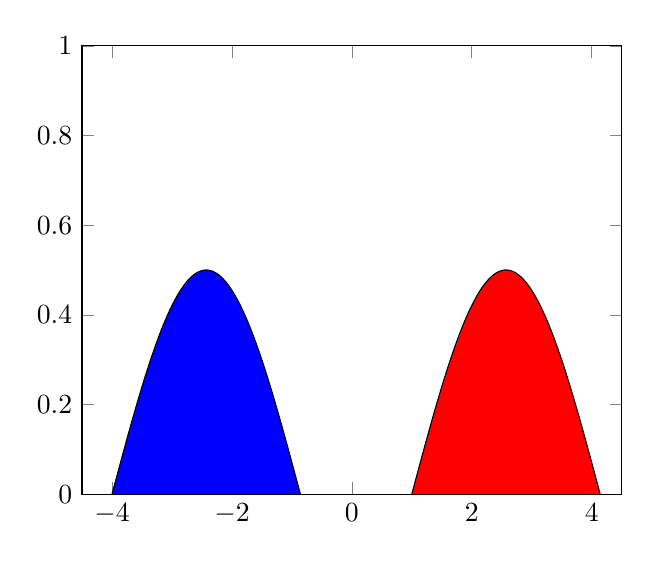
\begin{tikzpicture}
    \begin{axis}[ymin=0, ymax=1, xmin=-4.5, xmax=4.5]
      \addplot[domain=-4:-0.8584,samples=100,fill=blue]{sin(deg(x+4))/2};
      \addplot[domain=1:4.1416,samples=100, fill=red]{sin(deg(x-1))/2};
      \end{axis}
  \end{tikzpicture}
  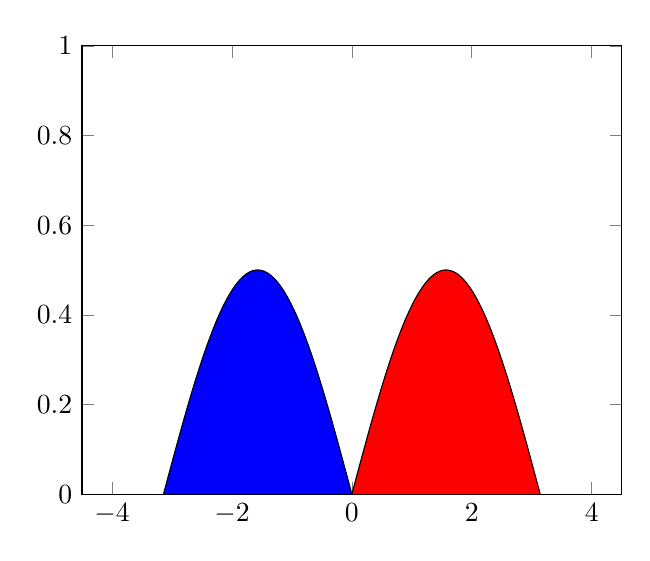
\begin{tikzpicture}
    \begin{axis}[ymin=0, ymax=1, xmin=-4.5, xmax=4.5]
      \addplot[domain=-3.1416:0,samples=100,fill=blue]{sin(deg(x+3.1416))/2};
      \addplot[domain=0:3.1416,samples=100, fill=red]{sin(deg(x))/2};
    \end{axis}
  \end{tikzpicture}
  % \missingfigure{two probability distributions moving closer together but same distance}
  \caption{Example of two different probability distances. 
    Even though the probability distributions of the second plot are closer than the ones on the first plot, they have the same distance in the $L^p$ norm.}
  \label{fig:example-wrong-distance}
\end{figure}
